%!TEX root = tcc_final.tex
\chapter{Framework de Desenvolvimento}\label{chap3:framework_desenvolvimento}
    
    % Referência para este capítulo é a própria documentação do ROS: http://wiki.ros.org/
    % Paper sobre ROS (não foi usado como referência, botei aqui apenas para manter o link): http://www.robotics.stanford.edu/~ang/papers/icraoss09-ROS.pdf
    
    Neste capítulo serão apresentadas as ferramentas utilizadas para o desenvolvimento deste trabalho, as funcionalidades que foram exploradas de cada uma delas e também detalhes importantes para o entendimento do desenvolvimento do trabalho.
    
    \section{Robot Operating System - ROS} \label{subchap3:ros}
        O sistema operacional robótico (do inglês \textit{"Robot Operating System"} - ROS) é um meta sistema operacional de código aberto mantido pelos esforços da comunidade internacional de pesquisadores em robótica. Um meta sistema operacional é um sistema que provê funcionalidades características de um sistema operacional porém é hospedado e executado pelo sistema operacional existente na máquina em questão.
        O ROS possui funcionalidades como abstração de hardware, controle de periféricos, troca de mensagens entre processos e etc, porém não possui autonomia sobre escalonamento, gerenciamento de memória e demais atividades que ficam a cargo do sistema operacional hospedeiro. O ROS pode ser compreendido como uma rede de processos (nodos) que possuem algum fator de acoplamento. Esses nodos podem ser processados na mesma máquina ou em máquinas distintas. A comunicação entre esses nodos é realizada 
        através da infraestrutura fornecida pelo ROS, que contempla comunicação síncrona e assíncrona. Os principais conceitos do ROS necessários para o entendimento deste trabalho são explicados a seguir:
        
        \begin{enumerate}[label=\Alph*]
            \item \textbf{Pacotes:} conjunto de nodos, bibliotecas, arquivos de configuração e etc que pode ser distribuído e integrado em sistemas distintos;
            \item \textbf{Nodos:} são os processos que formam o pacote. Cada processo pode ser um executável ou então um executável pode conter múltiplos processos.
            \item \textbf{Tópicos:} funcionalidade oferecida pelo ROS para troca de mensagens em uma abordagem publicador/inscrito (do inglês \textit{publisher/subscriber}). Comunicação N para N onde publicadores disponibilizam uma informação no tópico para possível consumo dos inscritos. Comunicação ocorre de forma não bloqueante, caracterizando uma comunicação assíncrona. % Encontrar referência para comunicação não bloqueante = assíncrona
            \item \textbf{Serviços:} funcionalidade oferecida pelo ROS para troca de mensagens em uma abordagem requisição e resposta. Essa comunicação ocorre de forma bloqueante, caracterizando uma comunicação síncrona. % Encontrar referência para comunicação bloqueante = síncrona
            \item \textbf{Bags:} formato do arquivo utilizando pelo ROS para gravar informações publicadas nos tópicos pelos nodos. Eficaz ferramenta para análise de execuções realizadas.
        \end{enumerate}
    
        
    
    \section{Sistema Base} \label{subchap3:sistema_base}
        O desenvolvimento deste trabalho foi realizado a partir do sistema implementado por Jurak~\cite{Jurak2020COLREGS}, que consiste em um sistema autônomo para veículos não tripulados que navegam na superfície da água (do inglês \textit{"Unmanned Surface Vehicle"} - USV) em conformidade com as regulamentações de prevenção de colisões no mar (do inglês \textit{"COLlision REGulations at Sea"} - COLREGS)~\cite{COLREGS}. Esse sistema foi implementado considerando que apenas embarcações de propulsão participarão do encontro e, além do veículo que terá o sistema de Jurak~\cite{Jurak2020COLREGS} embarcado, somente uma outra embarcação estará no mesmo cenário que o USV. Como ilustrado pela Figura~\ref{fig:chap2_arquitetura_base}, o sistema de Jurak~\cite{Jurak2020COLREGS} é composto basicamente por um pacote ROS chamado \textit{"mission planner"} que é responsável por gerar os objetivos (posição alvo) para o USV; um módulo chamado \textit{"Gazebo"} que consiste em um simulador robótico utilizado pelo USV\_sim\footnote{\url{https://github.com/disaster-robotics-proalertas/usv\_sim\_lsa}}~\cite{Paravisi2018Toward} para interagir com as embarcações; e um sistema de guia, navegação e controle (do inglês \textit{"Guidance, Navigation and Control} - GNC), sendo este o principal componente do sistema.
        
        \begin{figure}
            \centering
            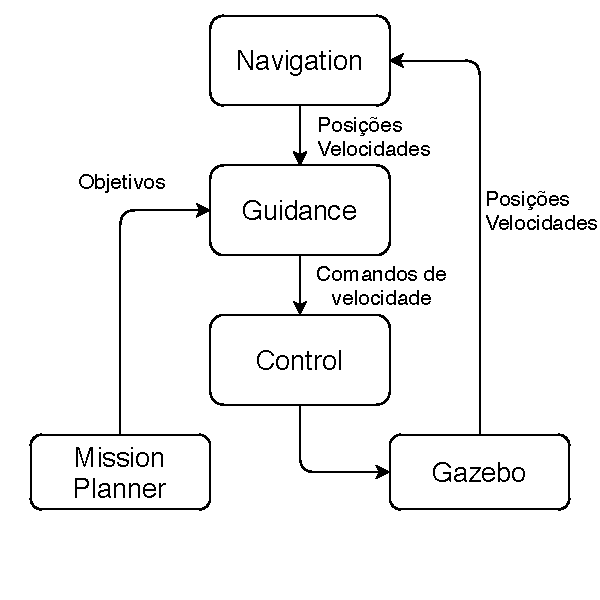
\includegraphics{fig/chap2/arquitetura_base.pdf}
            \caption{Arquitetura do sistema base}
            \label{fig:chap2_arquitetura_base}
        \end{figure}
        
        No sistema GNC desenvolvido por Jurak~\cite{Jurak2020COLREGS}, o entendimento do subsistema \textit{"Guidance"} é o de maior relevância para a compreensão deste trabalho. Como explicado no Capítulo~\ref{subchap2:USV}, o subsistema \textit{"Guidance"} é, em suma, responsável por determinar o caminho a ser seguido pelo USV, gerando comandos de velocidade para o subsistema \textit{"Control"}. O subsistema \textit{"Guidance"} desenvolvido por Jurak~\cite{Jurak2020COLREGS} conta com 2 planejadores, que são algoritmos responsáveis por determinar uma trajetória até uma posição alvo, ambos foram desenvolvidos a partir do pacote ROS chamado \textit{"move\_base"}. Um dos planejadores atua em escopo global (chamado de planejador global), realizando o planejamento da rota (rota global) a partir da posição em que o USV se encontra, até a posição objetivo (objetivo global). A rota global é planejada desviando de obstáculos estáticos (pontes, pedras, ilhas, corais) conhecidos a partir de mapas, cartas náuticas e etc. Já o outro planejador atua em escopo local (chamado de planejador local), sendo responsável pelo comportamento reativo à obstáculos que se aproximam. O planejador local determina o trajeto de curta 
        distância a ser percorrido pelo USV (rota local), desviando da rota global para que seja possível evitar um obstáculo que se aproxima e então retornar para a rota global. A posição alvo do planejador local (objetivo local) é a mais próxima possível da rota global, dentro do mapa local.

       O subsistema de \textit{"Guidance"} também conta com dois mapas de custo, que são representações virtuais do cenário onde o USV se encontra. Um dos mapas representa o cenário como um todo, denominado mapa global, enquanto que o outro mapa representa o entorno do USV, denominado mapa local. Para o caso do sistema de Jurak~\cite{Jurak2020COLREGS}, o mapa local representa uma área de 20mx20m com o USV localizado no centro dele. Os mapas são divididos em linhas e colunas, formando células onde cada uma possui um custo de 0 a 255. Uma célula com custo 0 indica que ela está totalmente livre e o USV consegue passar por ela. Já uma célula com custo 255 indica que a célula está totalmente obstruída e o USV não consegue passar por ela. Com isso, o planejador global e o planejador local podem determinar suas respectivas rotas através das células livres do mapa global e do mapa local. Como o planejador local é responsável pelo comportamento reativo do sistema, ele também é responsável por fazer com que o USV realize um desvio que atenda às requisições das COLREGS. Tais requisições são atendidas através da técnica de custo de terreno artificial (do inglês \textit{"Artificial Terrain Cost"} - ATC), que consiste em criar obstáculos virtuais na região que o USV não pode desviar, dado que essa seria uma região que viola as requisições da COLREGS, fazendo com o planejador local defina uma rota local por uma área que esteja em conformidade com as COLREGS. Esses obstáculos são criados a partir da embarcação que se aproxima até a borda do mapa local. Os obstáculos virtuais consistem em aumentar o custo das células do mapa local em que serão criadas, impossibilitando o planejador local de determinar uma rota que passe pelas células em questão. 
       
       Jurak~\cite{Jurak2020COLREGS} apresenta a Figura~\ref{fig:chap3_sistema_base_costmaps} que ilustra de forma completa os conceitos aqui apresentados. As regiões em tons de cinza indicam o mapa global, onde as células pretas representam obstáculos estáticos que não podem ser transpassados pelo USV. A região azul no entorno do USV (na imagem legendado como \textit{"Own Vessel"}) indica o mapa local, onde as células avermelhadas indicam obstáculos próximos que não podem ser transpassados pelo USV. É possível notar que a outra embarcação (na imagem legendada como \textit{"Encountering Vessel"}) está assinalado como um obstáculo. Também é possível notar a rota global (linha vermelha que parte do USV e vai para além do mapa local) se estendendo até o objetivo global. O objetivo local está indicado na borda do mapa local no ponto mais próximo possível da rota global. A imagem em questão está representando uma localização real, sendo esta o Arroio do Dilúvio na cidade de Porto Alegre no Rio Grande do Sul, Brasil.
       
       \begin{figure}
           \centering
           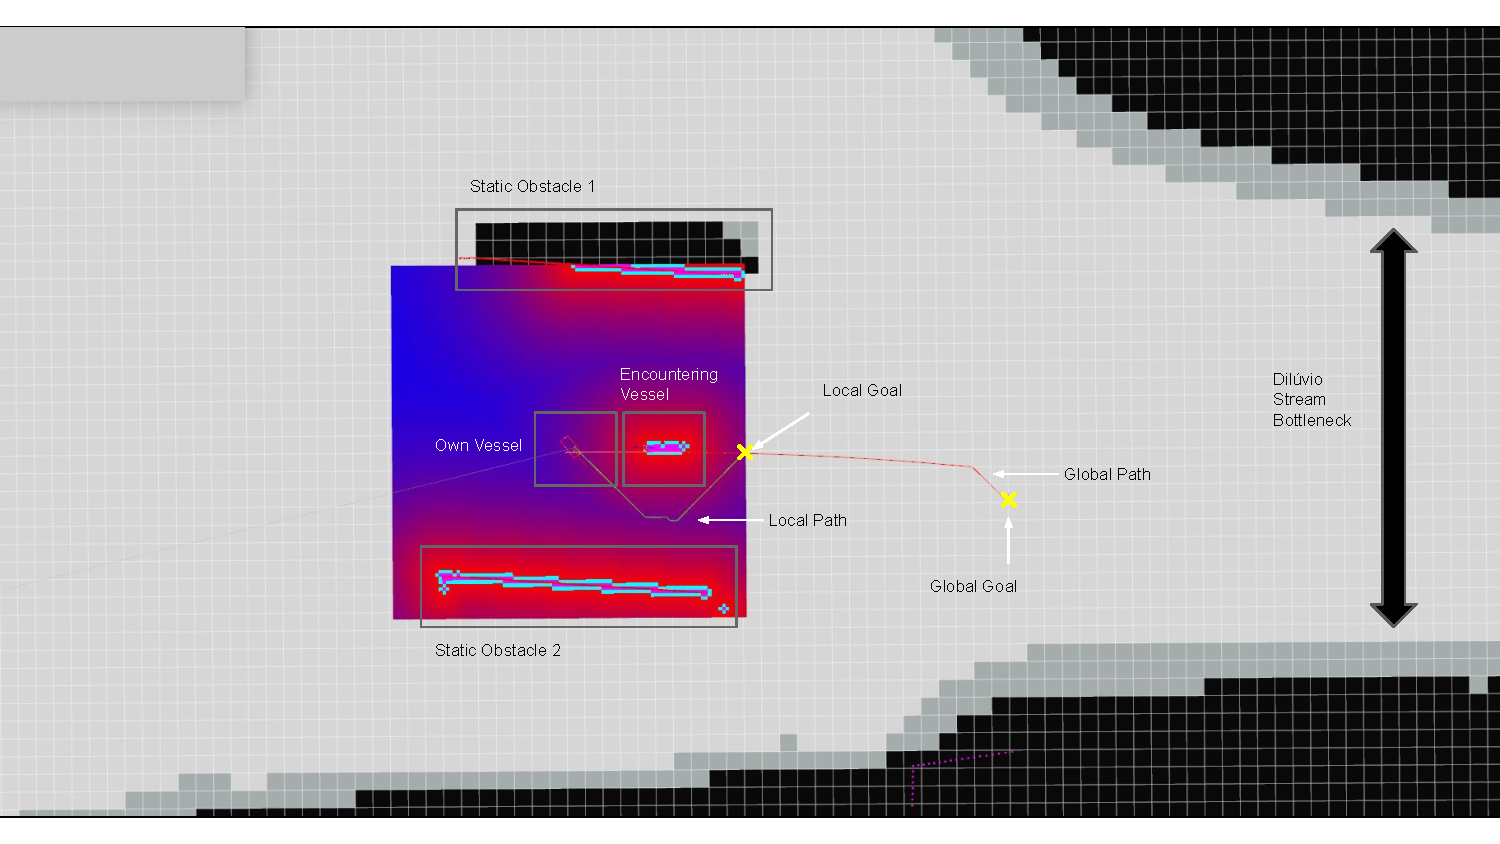
\includegraphics[scale=0.65]{fig/chap3/costmaps.pdf}
           \caption{Imagem apresentada por Jurak~\cite{Jurak2020COLREGS} ilustrando mapa global, mapa local, obstáculos, objetivo global, objetivo local, rota global e rota local}
           \label{fig:chap3_sistema_base_costmaps}
       \end{figure}